% genefinder pipeline overview.
% Build (from docs/figures/):
%   tectonic pipeline.tex                                   (XeLaTeX; or: xelatex pipeline.tex)
%   pdftocairo -svg pipeline.pdf pipeline.svg
%   pdftocairo -png -r 200 -singlefile pipeline.pdf pipeline
\documentclass[tikz,border=4pt]{standalone}
\usepackage{fontspec}
\setmainfont{texgyreheros}[Extension=.otf, UprightFont=*-regular, BoldFont=*-bold,
  ItalicFont=*-italic, BoldItalicFont=*-bolditalic]
\setmonofont{texgyrecursor}[Extension=.otf, UprightFont=*-regular, BoldFont=*-bold,
  ItalicFont=*-italic, BoldItalicFont=*-bolditalic]
\hyphenpenalty=10000 \exhyphenpenalty=10000
\usetikzlibrary{positioning,arrows.meta,shapes.geometric,fit,backgrounds,calc}

\definecolor{datac}{HTML}{2B6CB0}   % public inputs
\definecolor{setupc}{HTML}{6B7280}  % one-time setup
\definecolor{stepc}{HTML}{2C7A7B}   % per-run steps
\definecolor{outc}{HTML}{2F855A}    % outputs
\definecolor{genec}{HTML}{DD6B20}   % gene
\definecolor{flagc}{HTML}{C53030}   % QC flag

\tikzset{
  >={Stealth[length=2.4mm]},
  data/.style={cylinder, shape border rotate=90, aspect=0.16, draw=datac, thick, fill=datac!7,
               minimum width=3.7cm, minimum height=1.7cm, align=center, font=\scriptsize, text width=3.55cm},
  idx/.style={rectangle, rounded corners=3pt, draw=setupc, thick, fill=setupc!10, align=center,
              font=\scriptsize, text width=3.7cm, minimum height=1.2cm},
  stage/.style={rectangle, rounded corners=4pt, draw=stepc, very thick, fill=stepc!6, align=center,
                font=\scriptsize, text width=3.15cm, minimum height=2.7cm},
  stageout/.style={stage, draw=outc, fill=outc!7},
  num/.style={circle, fill=#1, text=white, font=\bfseries\small, inner sep=1.4pt, minimum size=5.2mm},
  flow/.style={->, very thick, stepc!80!black},
  feed/.style={->, thick, datac!85!black},
  lbl/.style={font=\tiny, inner sep=1.5pt, align=center},
  map/.style={gray!65, densely dashed, thin},
  section/.style={font=\scriptsize\bfseries, text=#1, rotate=90, anchor=center},
  band/.style={draw=none, fill=#1!5, rounded corners=6pt},
  gene/.style={fill=genec},
  contig/.style={fill=datac!30, rounded corners=1pt},
}
% gene arrow inside a gene box: \genearrow{x1}{x2}{y}
\newcommand{\genearrow}[3]{\draw[white, very thick, -{Stealth[length=1.3mm]}] (#1,#3) -- (#2,#3);}

\begin{document}
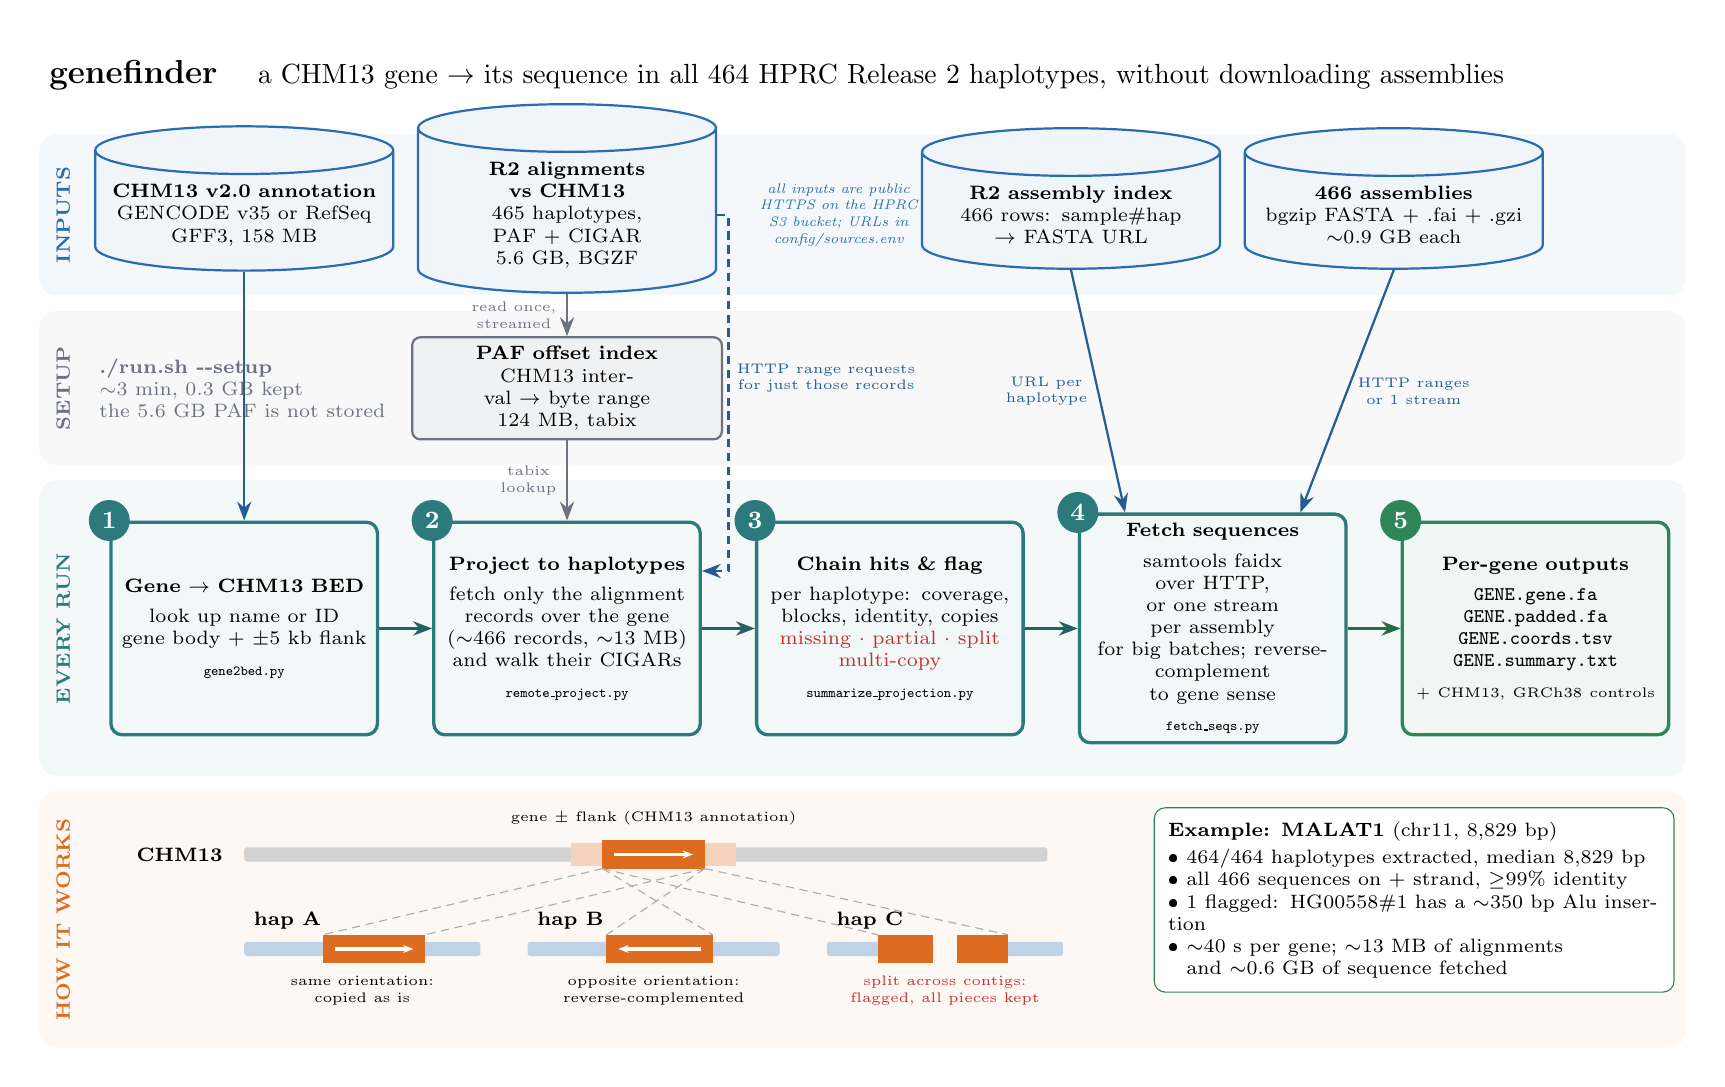
\begin{tikzpicture}
  % ---------------- background bands (also make the figure readable in dark mode) ----------------
  \begin{scope}[on background layer]
    \fill[white] (-2.75,1.55) rectangle (18.45,-11.55);
    \path[band=datac]  (-2.6,0.2)   rectangle (18.3,-1.85);
    \path[band=setupc] (-2.6,-2.05) rectangle (18.3,-4.0);
    \path[band=stepc]  (-2.6,-4.2)  rectangle (18.3,-7.95);
    \path[band=genec]  (-2.6,-8.15) rectangle (18.3,-11.4);
  \end{scope}
  \node[section=datac]  at (-2.3,-0.83) {INPUTS};
  \node[section=setupc] at (-2.3,-3.03) {SETUP};
  \node[section=stepc]  at (-2.3,-6.08) {EVERY RUN};
  \node[section=genec]  at (-2.3,-9.78) {HOW IT WORKS};

  % ---------------- title ----------------
  \node[anchor=west, font=\large] at (-2.6,0.95) {\textbf{genefinder}};
  \node[anchor=west, font=\normalsize] at (0.05,0.93)
    {a CHM13 gene \(\rightarrow\) its sequence in all 464 HPRC Release 2 haplotypes, without downloading assemblies};

  % ---------------- public inputs ----------------
  \node[data] (ann)  at (0,-0.83)    {\textbf{CHM13 v2.0 annotation}\\GENCODE v35 or RefSeq\\GFF3, 158 MB};
  \node[data] (paf)  at (4.1,-0.83)  {\textbf{R2 alignments vs CHM13}\\465 haplotypes, PAF + CIGAR\\5.6 GB, BGZF};
  \node[data] (aidx) at (10.5,-0.83) {\textbf{R2 assembly index}\\466 rows: sample\#hap\\\(\rightarrow\) FASTA URL};
  \node[data] (asm)  at (14.6,-0.83) {\textbf{466 assemblies}\\bgzip FASTA + .fai + .gzi\\\(\sim\)0.9 GB each};
  \node[lbl, font=\tiny\itshape, text=datac] at (7.55,-0.83)
    {all inputs are public\\HTTPS on the HPRC\\S3 bucket; URLs in\\config/sources.env};

  % ---------------- one-time setup ----------------
  \node[idx] (off) at (4.1,-3.03) {\textbf{PAF offset index}\\CHM13 interval \(\rightarrow\) byte range\\124 MB, tabix};
  \draw[->, thick, setupc] (paf.south) -- node[lbl, left=2pt, text=setupc] {read once,\\streamed} (off.north);
  \node[lbl, anchor=west, text=setupc, align=left, font=\scriptsize] at (-1.9,-3.03)
    {\textbf{./run.sh -{}-setup}\\\(\sim\)3 min, 0.3 GB kept\\the 5.6 GB PAF is not stored};

  % ---------------- per-run steps ----------------
  \node[stage] (s1) at (0,-6.08)
    {\textbf{Gene \(\rightarrow\) CHM13 BED}\\[3pt]look up name or ID\\gene body + \(\pm\)5 kb flank\\[3pt]{\tiny\ttfamily gene2bed.py}};
  \node[stage] (s2) at (4.1,-6.08)
    {\textbf{Project to haplotypes}\\[3pt]fetch only the alignment\\records over the gene\\(\(\sim\)466 records, \(\sim\)13 MB)\\and walk their CIGARs\\[3pt]{\tiny\ttfamily remote\_project.py}};
  \node[stage] (s3) at (8.2,-6.08)
    {\textbf{Chain hits \& flag}\\[3pt]per haplotype: coverage,\\blocks, identity, copies\\\textcolor{flagc}{missing \(\cdot\) partial \(\cdot\) split}\\\textcolor{flagc}{multi-copy}\\[3pt]{\tiny\ttfamily summarize\_projection.py}};
  \node[stage] (s4) at (12.3,-6.08)
    {\textbf{Fetch sequences}\\[3pt]samtools faidx over HTTP,\\or one stream per assembly\\for big batches; reverse-\\complement to gene sense\\[3pt]{\tiny\ttfamily fetch\_seqs.py}};
  \node[stageout] (s5) at (16.4,-6.08)
    {\textbf{Per-gene outputs}\\[3pt]{\ttfamily GENE.gene.fa}\\{\ttfamily GENE.padded.fa}\\{\ttfamily GENE.coords.tsv}\\{\ttfamily GENE.summary.txt}\\[3pt]{\tiny + CHM13, GRCh38 controls}};
  \node[num=stepc] at (s1.north west) {1};
  \node[num=stepc] at (s2.north west) {2};
  \node[num=stepc] at (s3.north west) {3};
  \node[num=stepc] at (s4.north west) {4};
  \node[num=outc]  at (s5.north west) {5};

  \draw[flow] (s1) -- (s2);
  \draw[flow] (s2) -- (s3);
  \draw[flow] (s3) -- (s4);
  \draw[flow, outc!80!black] (s4) -- (s5);

  % inputs feeding the steps
  \draw[feed] (ann.south) -- (s1.north);
  \draw[feed, setupc] (off.south) -- node[lbl, left=2pt, text=setupc] {tabix\\lookup} (s2.north);
  \draw[feed, densely dashed] (paf.east) -| (6.15,-5.35) -- ($(s2.east)+(0,0.73)$);
  \node[lbl, text=datac!85!black, anchor=west] at (6.2,-2.9) {HTTP range requests\\for just those records};
  \draw[feed] (aidx.south) -- node[lbl, left=2pt, pos=0.5, text=datac!85!black] {URL per\\haplotype} ($(s4.north west)+(0.6,0)$);
  \draw[feed] (asm.south) -- node[lbl, right=2pt, pos=0.5, text=datac!85!black] {HTTP ranges\\or 1 stream} ($(s4.north east)+(-0.6,0)$);

  % ---------------- projection schematic ----------------
  \def\yC{-8.95}
  \def\yH{-10.15}
  % CHM13
  \node[font=\scriptsize\bfseries, anchor=east] at (-0.15,\yC) {CHM13};
  \fill[gray!35, rounded corners=1pt] (0,\yC-0.09) rectangle (10.2,\yC+0.09);
  \fill[genec!30] (4.15,\yC-0.15) rectangle (4.55,\yC+0.15);
  \fill[genec!30] (5.85,\yC-0.15) rectangle (6.25,\yC+0.15);
  \fill[gene] (4.55,\yC-0.18) rectangle (5.85,\yC+0.18); \genearrow{4.7}{5.7}{\yC}
  \node[font=\tiny, above=2pt] at (5.2,\yC+0.18) {gene \(\pm\) flank (CHM13 annotation)};
  % hap A: forward
  \node[font=\scriptsize\bfseries, anchor=south west] at (0,\yH+0.12) {hap A};
  \fill[contig] (0,\yH-0.09) rectangle (3.0,\yH+0.09);
  \fill[gene] (1.0,\yH-0.18) rectangle (2.3,\yH+0.18); \genearrow{1.15}{2.15}{\yH}
  \draw[map] (4.55,\yC-0.18) -- (1.0,\yH+0.18);  \draw[map] (5.85,\yC-0.18) -- (2.3,\yH+0.18);
  \node[font=\tiny, anchor=north, align=center] at (1.5,\yH-0.22) {same orientation:\\copied as is};
  % hap B: reverse
  \node[font=\scriptsize\bfseries, anchor=south west] at (3.6,\yH+0.12) {hap B};
  \fill[contig] (3.6,\yH-0.09) rectangle (6.8,\yH+0.09);
  \fill[gene] (4.6,\yH-0.18) rectangle (5.95,\yH+0.18); \genearrow{5.8}{4.75}{\yH}
  \draw[map] (4.55,\yC-0.18) -- (5.95,\yH+0.18);  \draw[map] (5.85,\yC-0.18) -- (4.6,\yH+0.18);
  \node[font=\tiny, anchor=north, align=center] at (5.2,\yH-0.22) {opposite orientation:\\reverse-complemented};
  % hap C: split across two contigs
  \node[font=\scriptsize\bfseries, anchor=south west] at (7.4,\yH+0.12) {hap C};
  \fill[contig] (7.4,\yH-0.09) rectangle (8.75,\yH+0.09);
  \fill[contig] (9.05,\yH-0.09) rectangle (10.4,\yH+0.09);
  \fill[gene] (8.05,\yH-0.18) rectangle (8.75,\yH+0.18);
  \fill[gene] (9.05,\yH-0.18) rectangle (9.7,\yH+0.18);
  \draw[map] (4.55,\yC-0.18) -- (8.05,\yH+0.18);  \draw[map] (5.85,\yC-0.18) -- (9.7,\yH+0.18);
  \node[font=\tiny, anchor=north, align=center, text=flagc] at (8.9,\yH-0.22) {split across contigs:\\flagged, all pieces kept};

  % ---------------- example ----------------
  \node[draw=outc, rounded corners=4pt, fill=white, align=left, font=\scriptsize, anchor=north west,
        text width=6.25cm, inner sep=5pt] at (11.55,-8.35)
    {\textbf{Example: MALAT1} (chr11, 8,829 bp)\\[2pt]
     \textbullet\ 464/464 haplotypes extracted, median 8,829 bp\\
     \textbullet\ all 466 sequences on + strand, \(\ge\)99\% identity\\
     \textbullet\ 1 flagged: HG00558\#1 has a \(\sim\)350 bp Alu insertion\\
     \textbullet\ \(\sim\)40 s per gene; \(\sim\)13 MB of alignments\\\phantom{\textbullet\ }and \(\sim\)0.6 GB of sequence fetched};
\end{tikzpicture}
\end{document}
